\chapter{Gr'aficas}

%-----------------------------------------------------------
\section{Gr'aficas est'andar}

\begin{verbatim}
setwd("path")
credit <- read.csv(file = "../data/credit-g.csv", sep = ",", 
          na.strings = "NULL")
attach(credit)

set.seed(32) # Muestra
dsmall <- credit[sample(nrow(credit), 5), ]
dsmall
\end{verbatim}

%-----
\subsection{Puntos}

\begin{verbatim}
png(filename = "../figures/foo1.png") # puntos
plot(age,credit_amount)
\end{verbatim}

\begin{verbatim}
png(filename = "../figures/foo1b.png")
plot(dsmall$age,type= "o",col="blue")
\end{verbatim}

\begin{verbatim}
png(filename = "../figures/foo1c.png")
plot(dsmall$existing_credits, type="o", col="blue", ylim=c(0,12))
lines(dsmall$residence_since, type="o", pch=22, lty=2, col="red")
legend(7,12, c("existing_credits","residence_since"), 
   col=c("blue","red"), pch=21:22, lty=1:2)
\end{verbatim}

\begin{figure}[h]
 \begin{center}
 \subfigure[foo1]{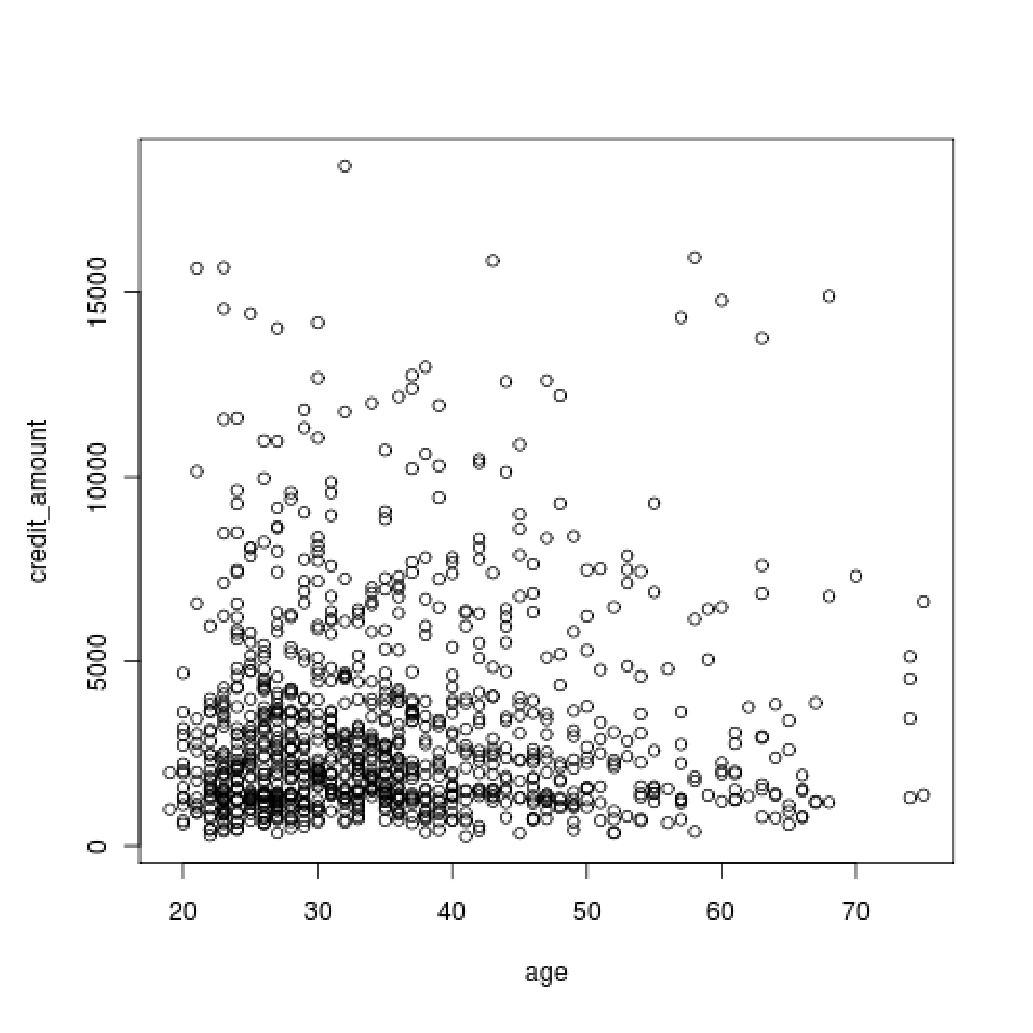
\includegraphics[keepaspectratio,width=4cm]{theimg/foo1}}
 \hspace{0.1cm}
 \subfigure[foo1b]{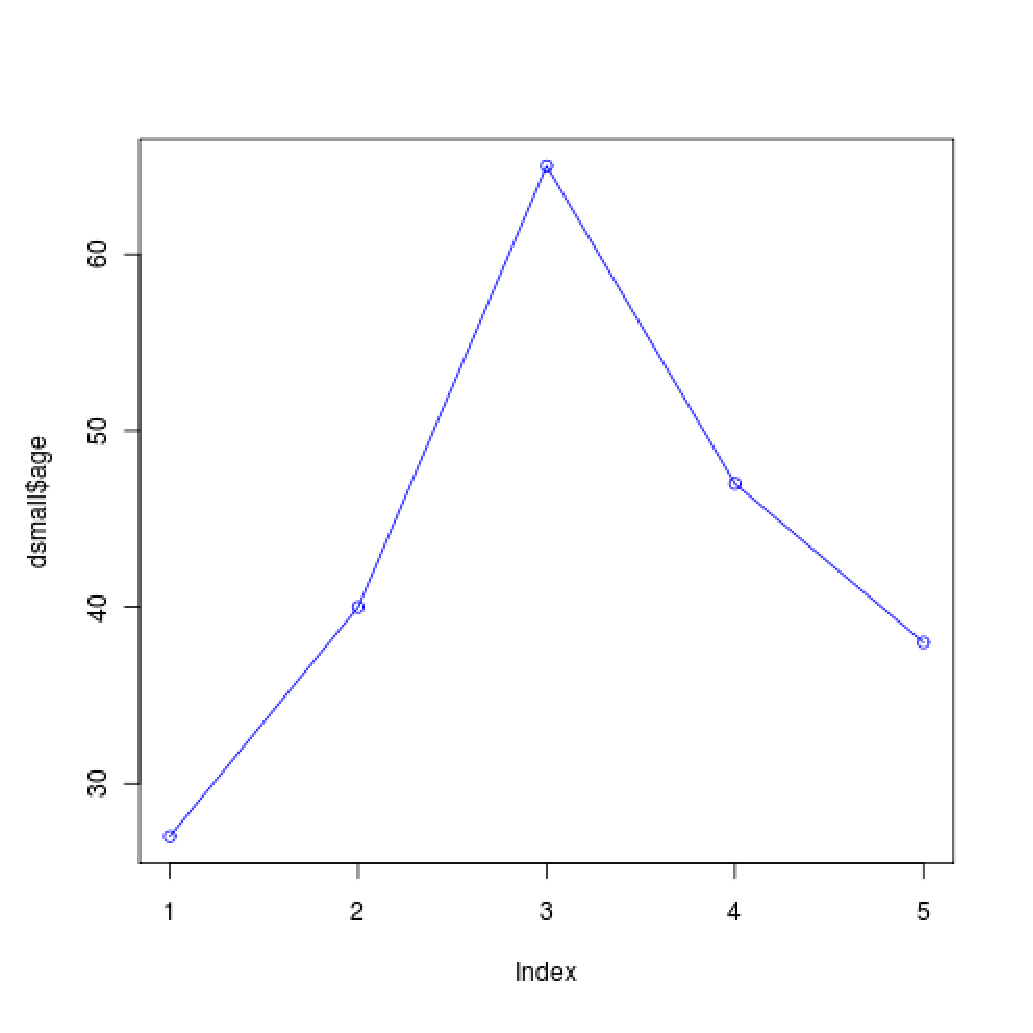
\includegraphics[keepaspectratio,width=4cm]{theimg/foo1b}}
 \hspace{0.1cm}
 \subfigure[foo1c]{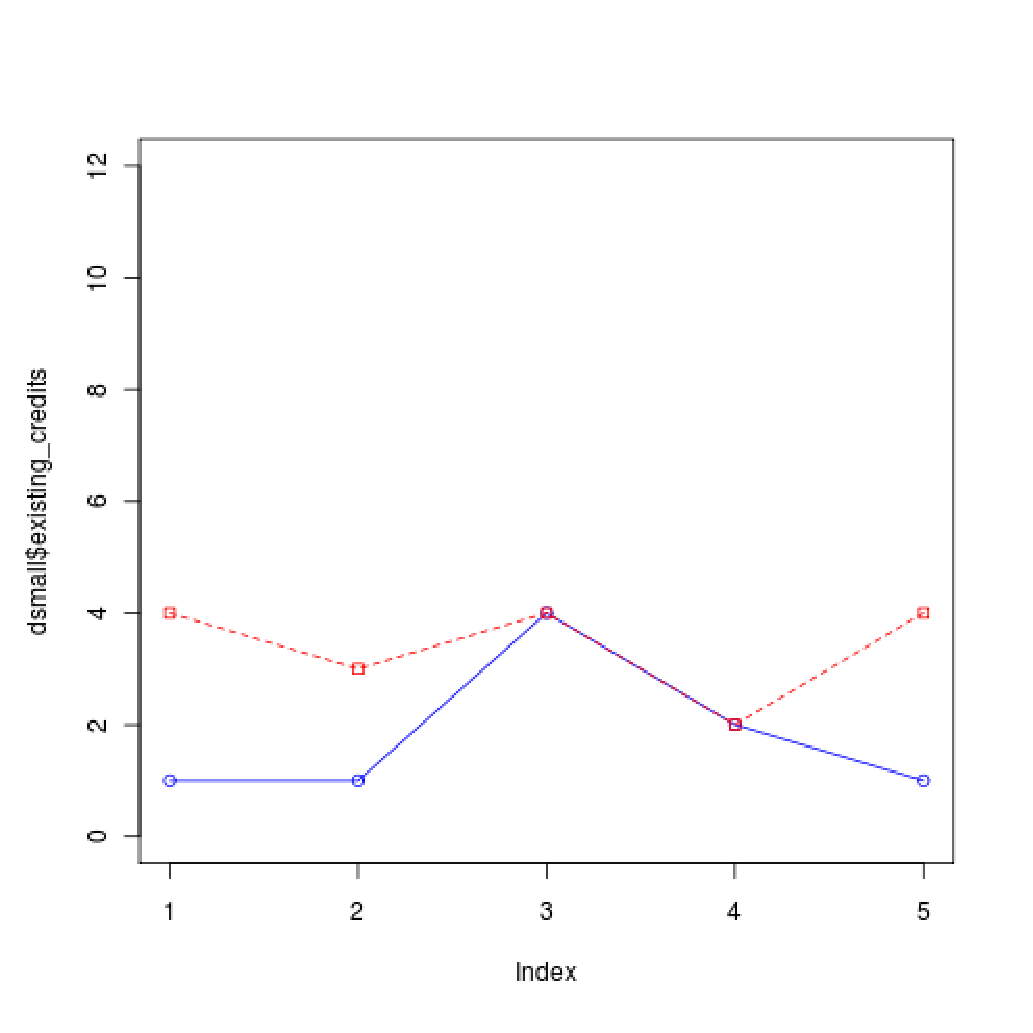
\includegraphics[keepaspectratio,width=4cm]{theimg/foo1c}}
 \caption{Puntos}
 \label{fig:puntos}
 \end{center}
\end{figure}

%-----
\subsection{Bigotes}

\begin{verbatim}
png(filename = "../figures/foo2.png")
boxplot(age)
\end{verbatim}

\begin{figure}[h]
 \centering
 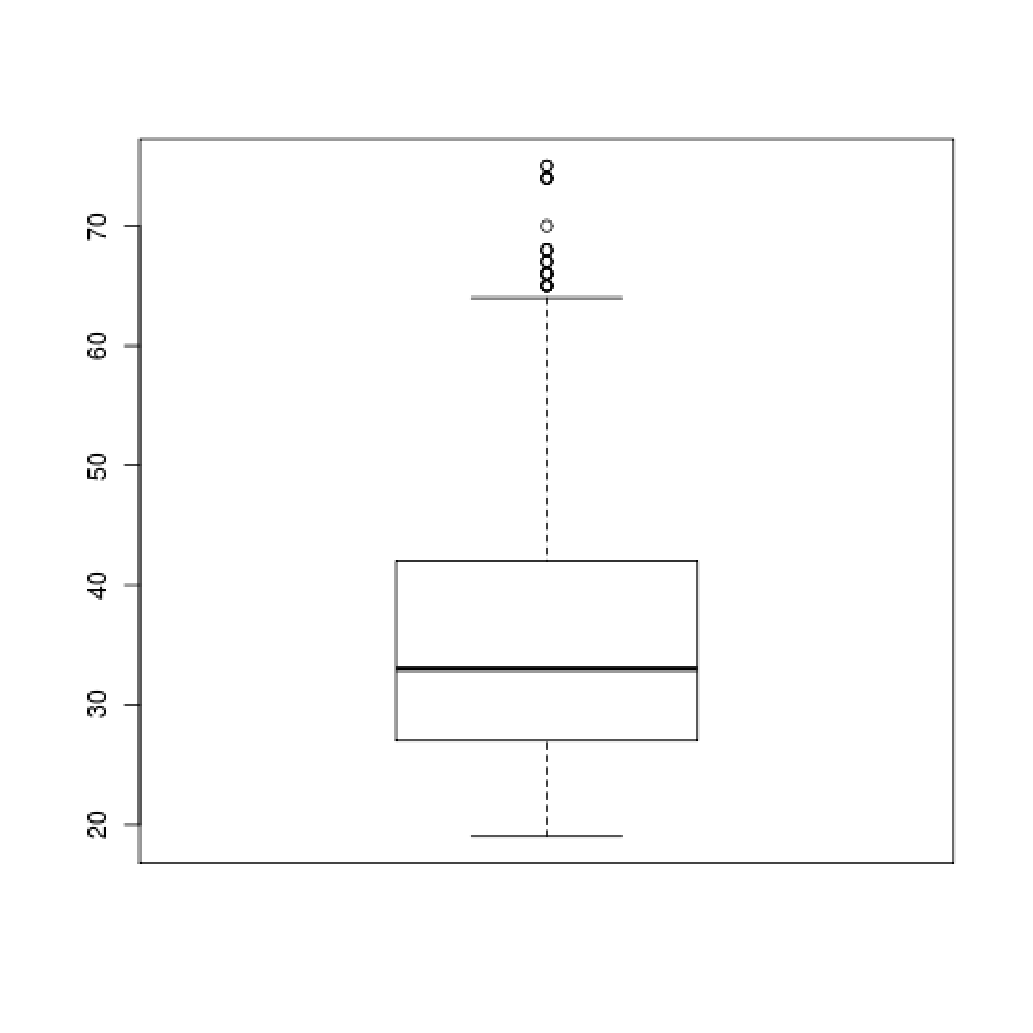
\includegraphics[keepaspectratio,width=5cm]{theimg/foo2}
 \caption[foo2]{foo2}
 \label{fig:bigos}
\end{figure}

%-----
\subsection{Histograma simple}

\begin{verbatim}
png(filename = "../figures/foo3.png")
hist(credit_amount)
\end{verbatim}

\begin{verbatim}
png(filename = "../figures/foo4.png")
hist(credit_amount, breaks=30, col="blue") 
\end{verbatim}

\begin{figure}[h]
 \begin{center}
 \subfigure[foo3]{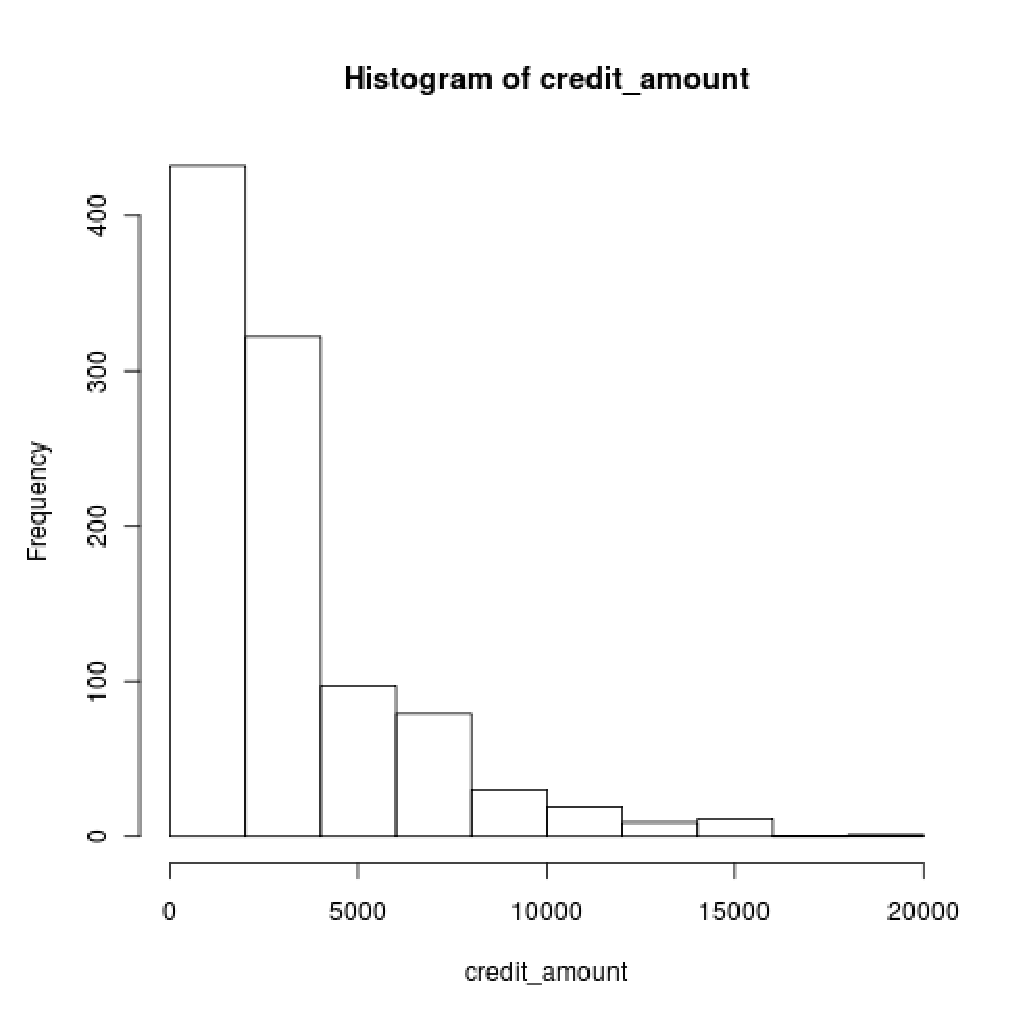
\includegraphics[keepaspectratio,width=6cm]{theimg/foo3}}
 \hspace{0.1cm}
 \subfigure[foo4]{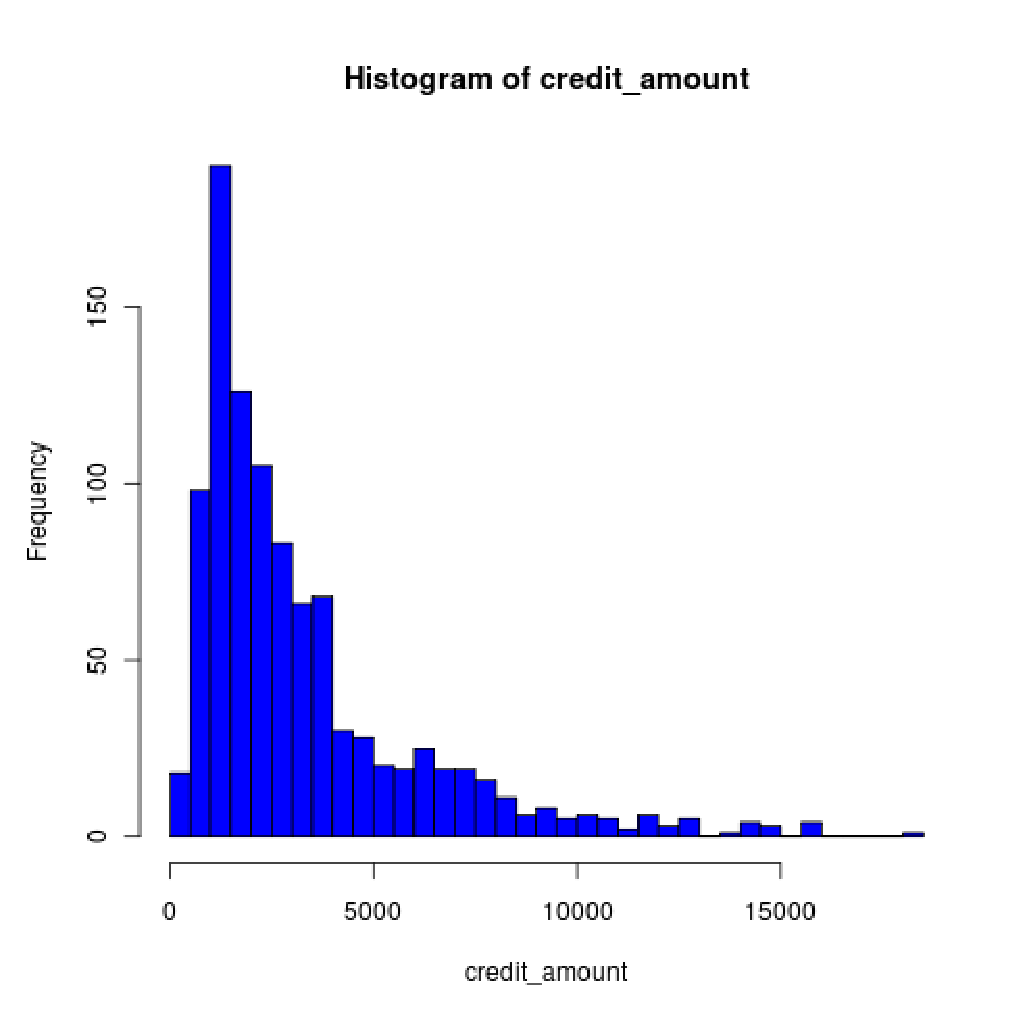
\includegraphics[keepaspectratio,width=6cm]{theimg/foo4}}
 \caption{Histograma}
 \label{fig:histograma}
 \end{center}
\end{figure}

%-----
\subsection{Barras}

\begin{verbatim}
png(filename = "../figures/foo5.png")
counts <- table(housing)
barplot(counts, main="Housing") 
\end{verbatim}

\begin{verbatim}
png(filename = "../figures/foo6.png")
counts <- table(class)
barplot(counts, main="Personal status", horiz=TRUE)
\end{verbatim}

\begin{verbatim}
png(filename = "../figures/foo6a.png")
myfile <- data.frame(dsmall$age,dsmall$residence_since,dsmall$duration)
barplot(as.matrix(myfile), main="Crédito", ylab= "Total",
   beside=TRUE, col=rainbow(5), cex.names=0.9)
legend("topright", c("e1","e2","e3","e4","e5"), bty="n", fill=rainbow(5))
\end{verbatim}

\begin{figure}[h]
 \begin{center}
 \subfigure[foo5]{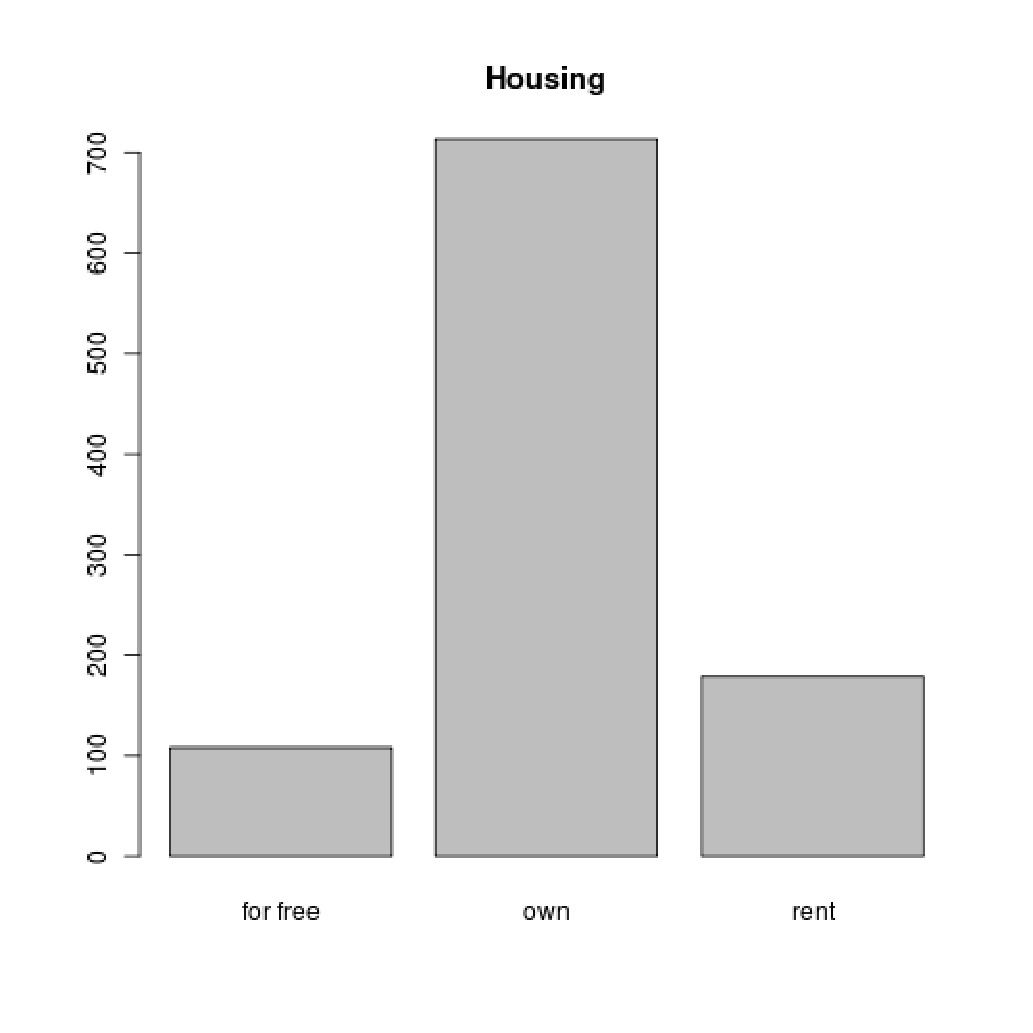
\includegraphics[keepaspectratio,width=4cm]{theimg/foo5}}
 \hspace{0.1cm}
 \subfigure[foo6]{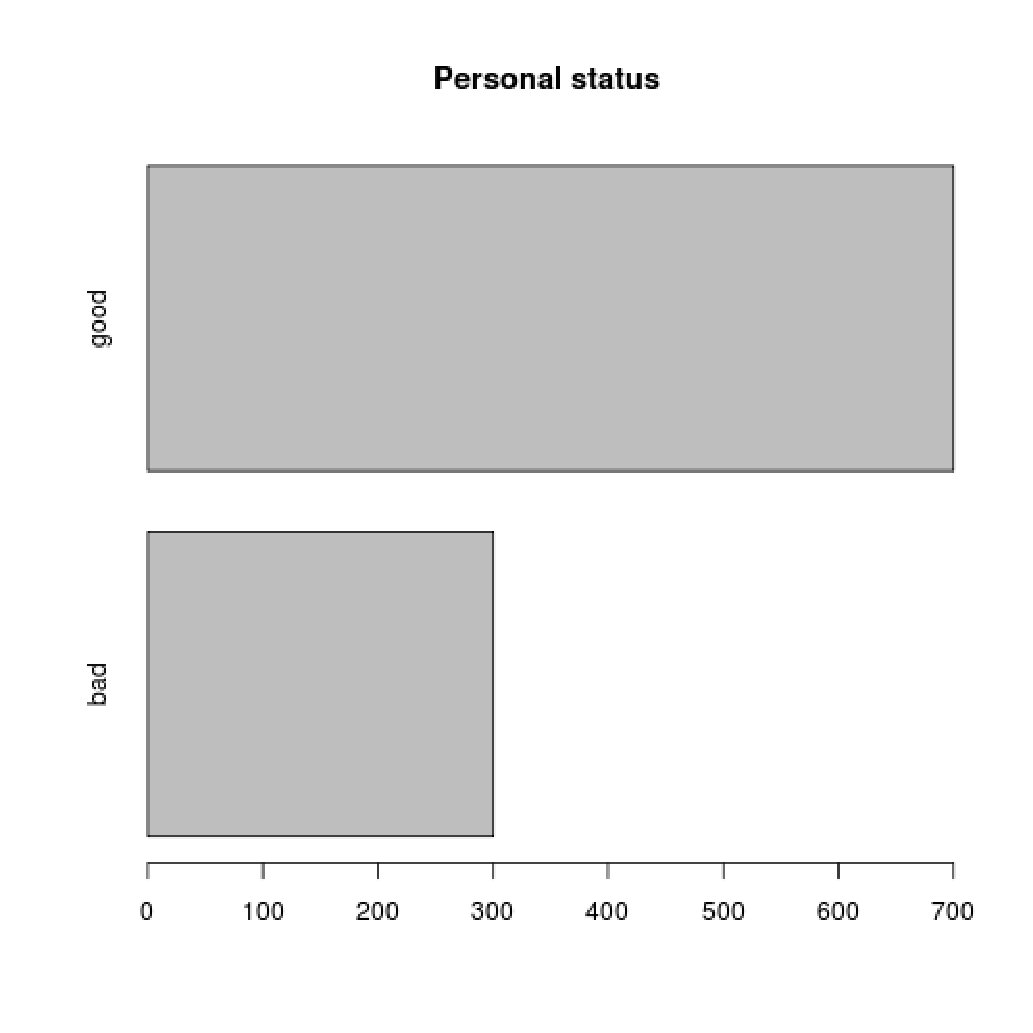
\includegraphics[keepaspectratio,width=4cm]{theimg/foo6}}
 \hspace{0.1cm}
 \subfigure[foo6a]{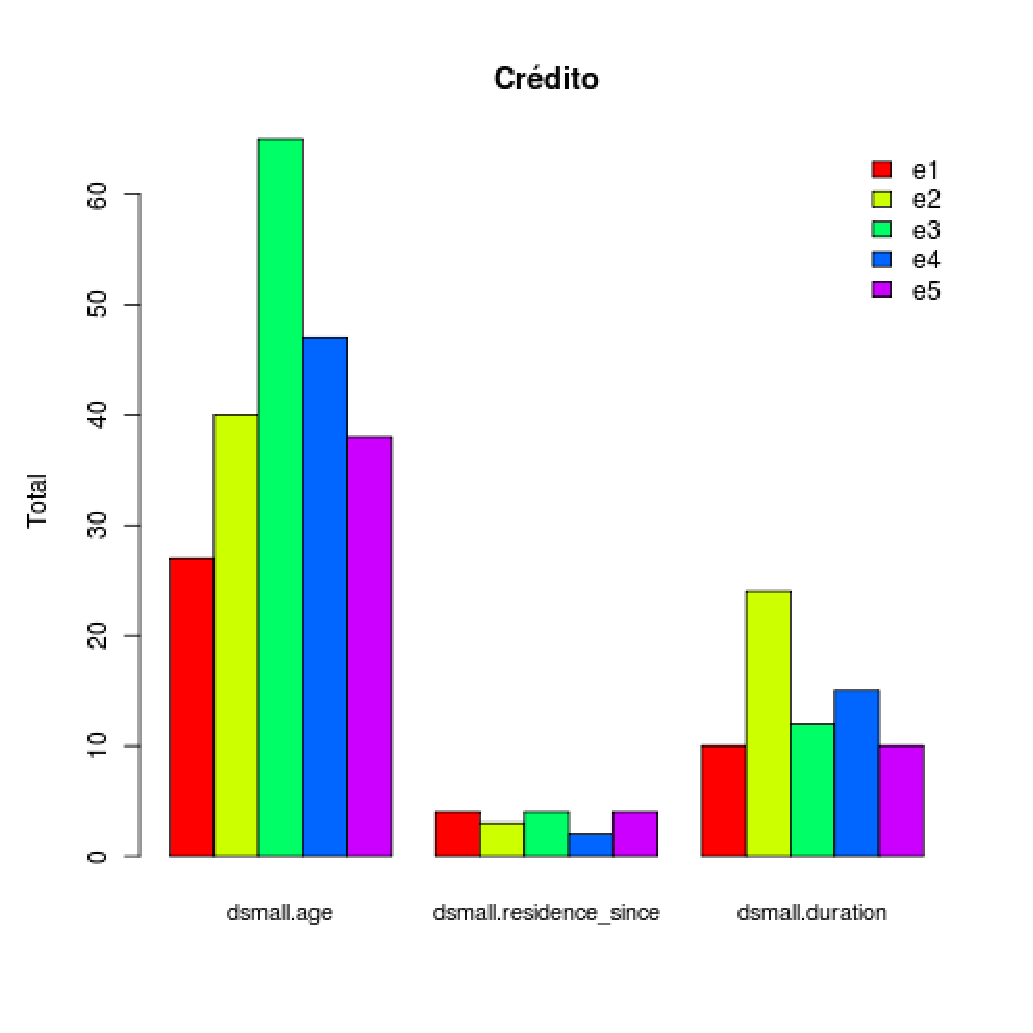
\includegraphics[keepaspectratio,width=4cm]{theimg/foo6a}}
 \caption{Barras}
 \label{fig:barras}
 \end{center}
\end{figure}

%-----
\subsection{Densidad}

\begin{verbatim}
png(filename = "../figures/foo7.png")
d <- density(credit_amount) # returns the density data
plot(d) # plots the results 
\end{verbatim}

\begin{verbatim}
png(filename = "../figures/foo8.png")
d <- density(credit_amount)
plot(d)
polygon(d, col="red") 
\end{verbatim}

\begin{figure}[h]
 \begin{center}
 \subfigure[foo7]{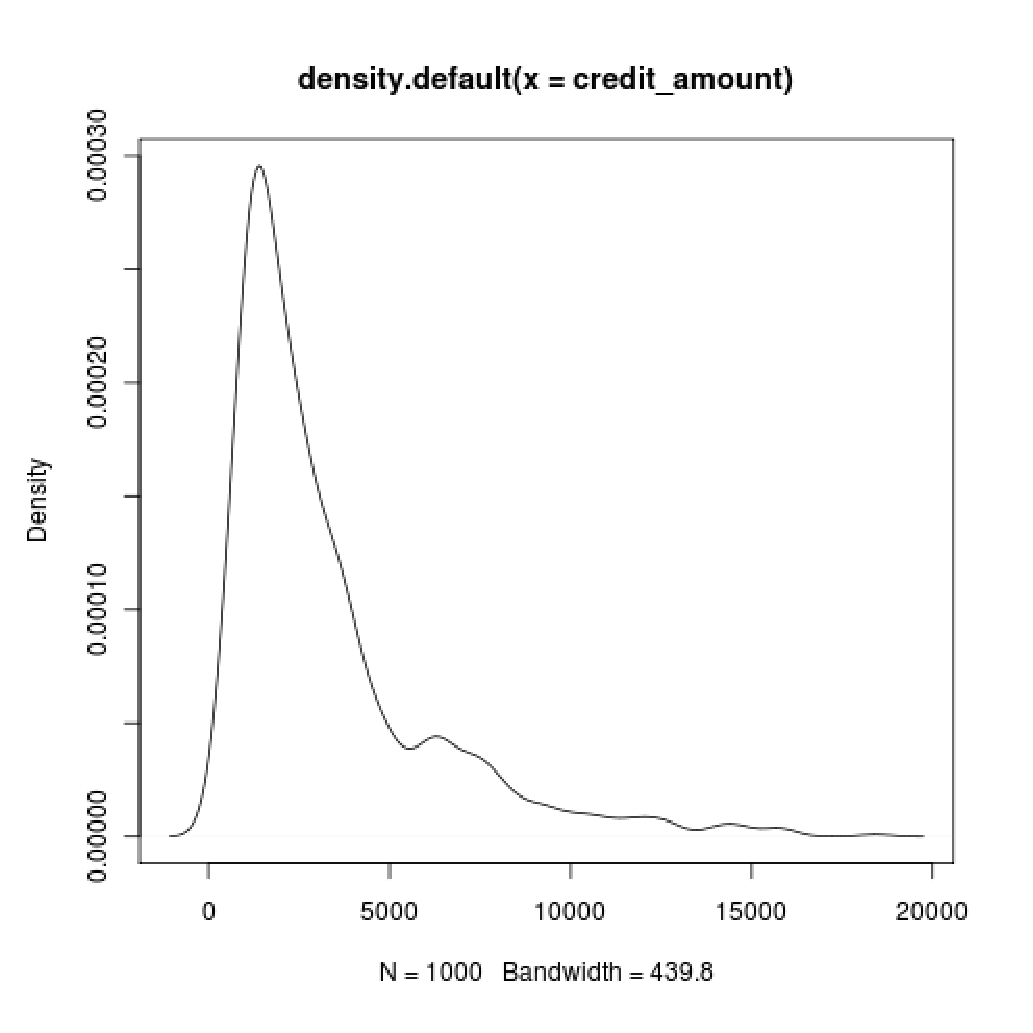
\includegraphics[keepaspectratio,width=5cm]{theimg/foo7}}
 \hspace{0.1cm}
 \subfigure[foo8]{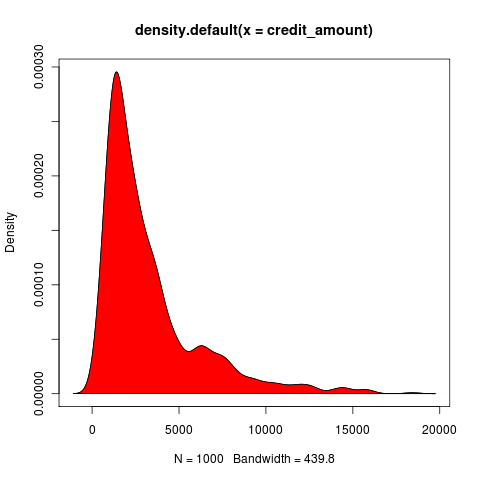
\includegraphics[keepaspectratio,width=5cm]{theimg/foo8}}
 \caption{Densidad}
 \label{fig:densidad}
 \end{center}
\end{figure}

%-----
\subsection{Matriz de dispersi'on}

\begin{verbatim}
png(filename = "../figures/foo9.png")
pairs(~credit_amount+age+existing_credits+num_dependents,data=credit,
   main="Simple Scatterplot Matrix")

\end{verbatim}

\begin{figure}[h]
 \centering
 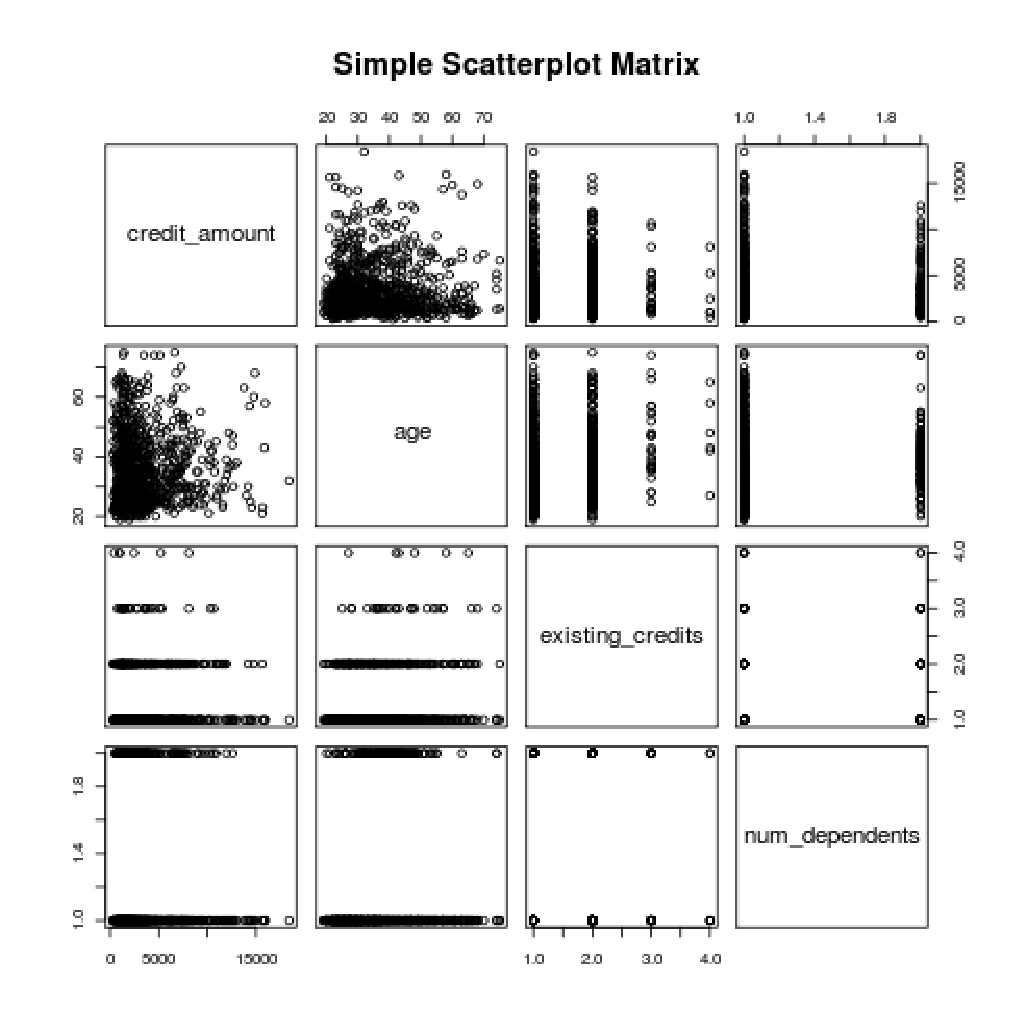
\includegraphics[keepaspectratio,width=7cm]{theimg/foo9}
 \caption[foo9]{foo9}
 \label{fig:puntos5}
\end{figure}


%-----------------------------------------------------------
\section{Librer'ia ggplot2}

%-----
\subsection{Bigotes}

\begin{verbatim}
d <- ggplot(data = credit, aes(x = credit_amount, y = age)) 
d + geom_boxplot(outlier.shape = 4) + theme_bw() + 
    scale_y_continuous(breaks = seq(0, 100, by = 5))
ggsave(file = "../figures/gg-boxplot.eps", width=5, height=5)
\end{verbatim}

%-----
\subsection{Barras}

\begin{verbatim}
d <- ggplot(data = credit, aes(age)) 
d + geom_bar() + theme_bw()
ggsave(file = "../figures/gg-foo10.eps", width=5, height=5)
\end{verbatim}

\begin{verbatim}
d <- ggplot(data = credit, aes(age)) 
d + geom_bar(binwidth = 0.1) + theme_bw()
ggsave(file = "../figures/gg-foo10a.eps", width=5, height=5)
\end{verbatim}

\begin{figure}[h]
 \begin{center}
 \subfigure[gg-boxplot]{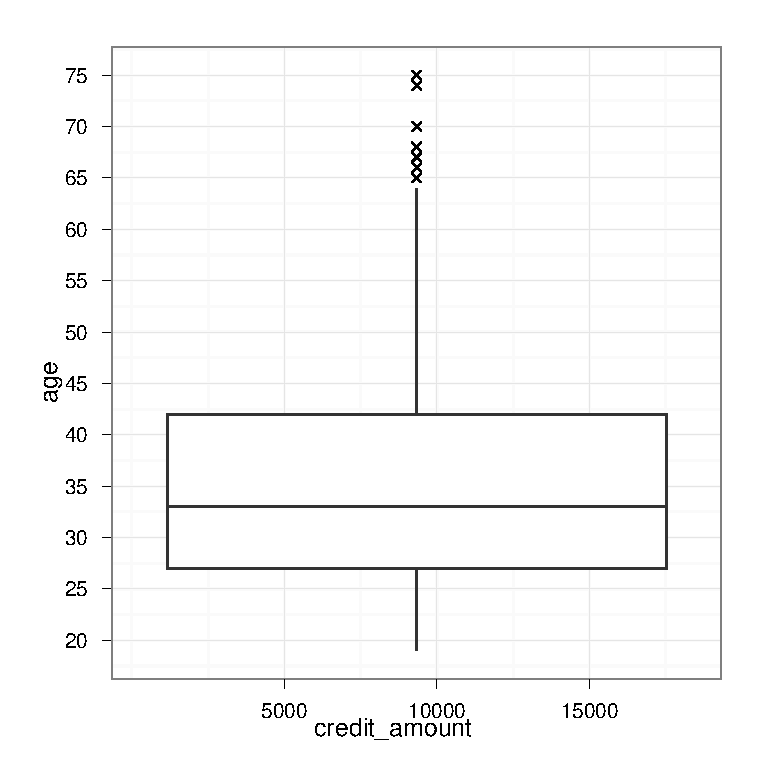
\includegraphics[keepaspectratio,width=4cm]{theimg/gg-boxplot}}
 \hspace{0.1cm}
 \subfigure[gg-foo10]{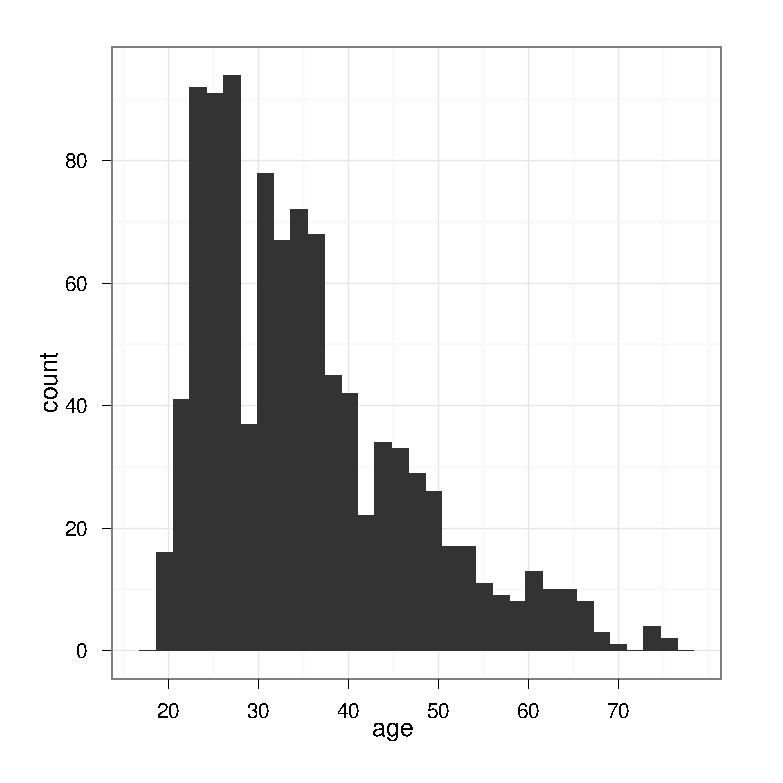
\includegraphics[keepaspectratio,width=4cm]{theimg/gg-foo10}}
 \hspace{0.1cm}
 \subfigure[gg-foo10a]{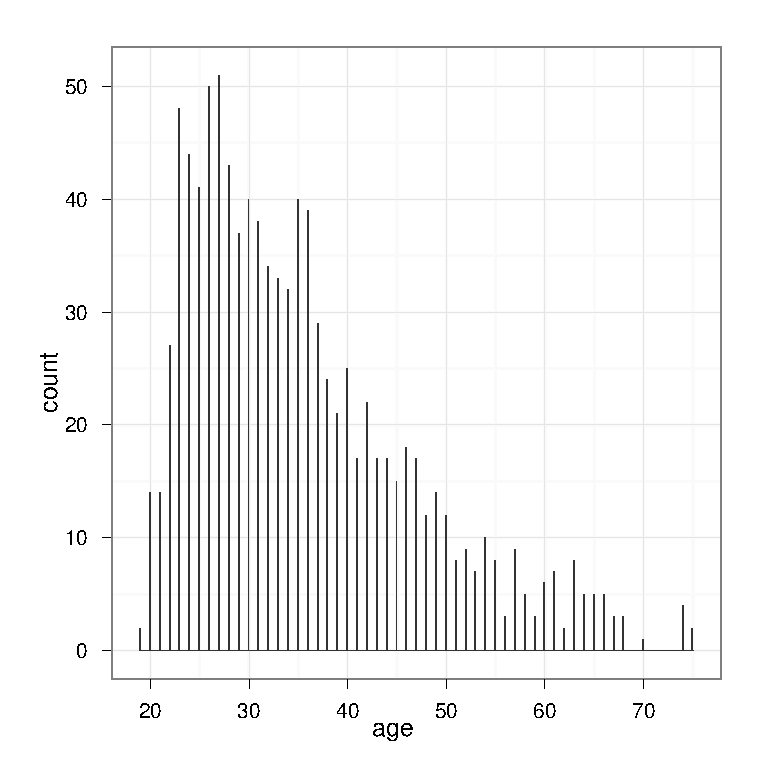
\includegraphics[keepaspectratio,width=4cm]{theimg/gg-foo10a}}
 \caption{Bigotes y barras}
 \label{fig:barras}
 \end{center}
\end{figure}

\begin{verbatim}
d <- ggplot(data = credit, aes(age)) 
d + geom_histogram(aes(y = ..count..),binwidth = 0.5)  + 
    theme_bw() + 
   scale_x_continuous(breaks = c(media)) + 
    geom_vline(xintercept = media, size = 0.5, colour = "magenta") +
    geom_vline(xintercept = media+sd, size = 0.5, colour = "blue", linetype = 2) +
    geom_vline(xintercept = media-sd, size = 0.5, colour = "blue", linetype = 2) 
ggsave(file = "../figures/gg-foo11.eps", width=5, height=5)
\end{verbatim}

\begin{figure}[h]
 \centering
 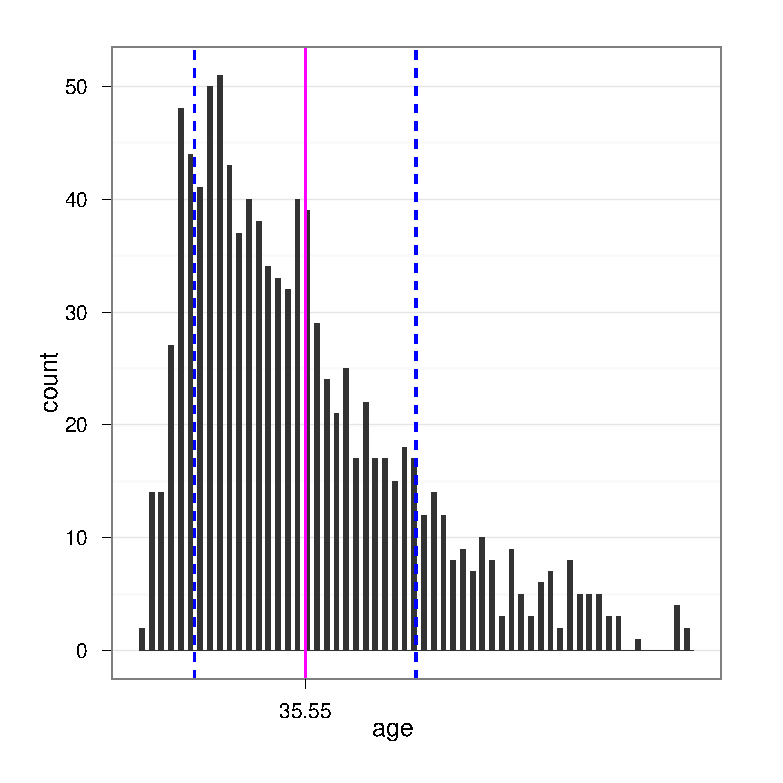
\includegraphics[keepaspectratio,width=6.5cm]{theimg/gg-foo11}
 \caption[foo11]{gg-foo11}
 \label{fig:foo11}
\end{figure}

\begin{verbatim}
agebin = cut(age,breaks = c(18,30,40,50,60,70,80))
agebinfile <- data.frame(purpose,credit_amount,personal_status,housing,job,
                         age=agebin,class)
agebinfile

d <- ggplot(data = agebinfile, aes(age)) 
d + stat_bin(aes(ymax = ..count..), geom = "bar") + theme_bw()
ggsave(file = "../figures/gg-foo12.eps", width=5, height=5)
\end{verbatim}

\begin{verbatim}
d <- ggplot(credit, aes(housing))
d + geom_bar()
ggsave(file = "../figures/gg-foo13.eps", width=5, height=5)
\end{verbatim}

\begin{figure}[h]
 \begin{center}
 \subfigure[gg-foo12]{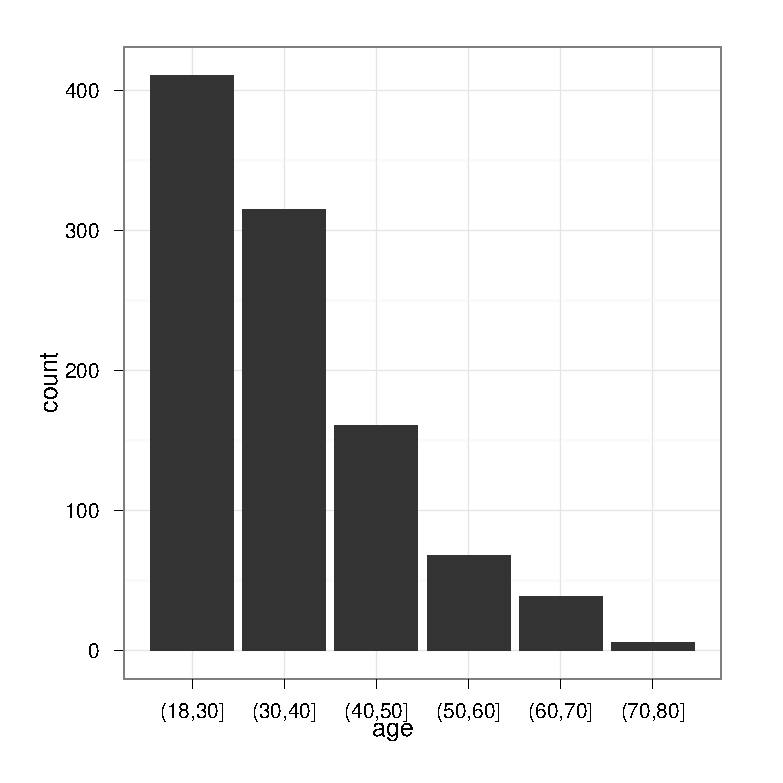
\includegraphics[keepaspectratio,width=5cm]{theimg/gg-foo12}}
 \hspace{0.1cm}
 \subfigure[gg-foo13]{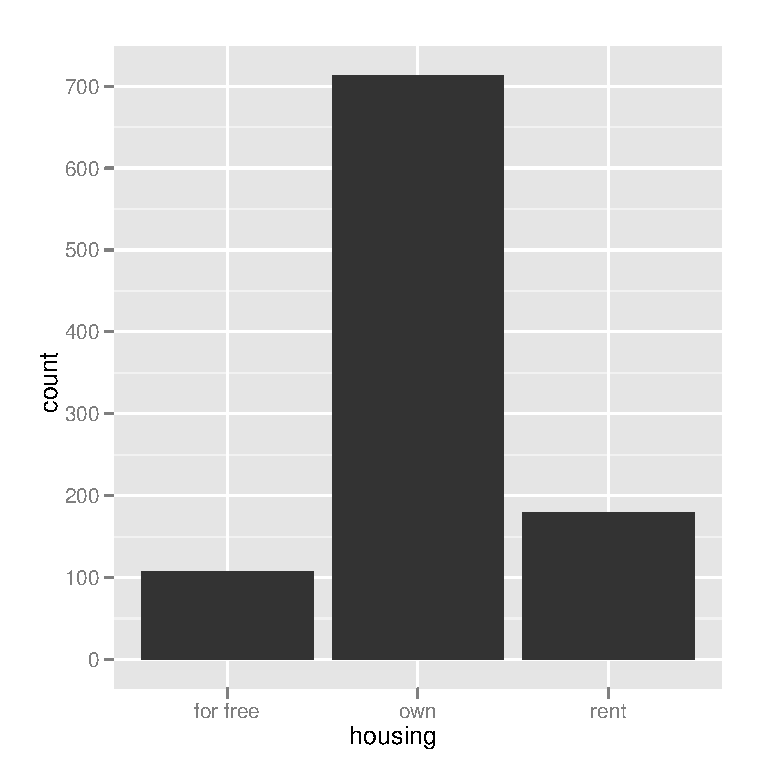
\includegraphics[keepaspectratio,width=5cm]{theimg/gg-foo13}}
 \caption{Barras}
 \label{fig:barras}
 \end{center}
\end{figure}

\begin{verbatim}
d <- ggplot(credit, aes(age,fill=housing))
d + geom_bar()
ggsave(file = "../figures/gg-foo14.eps", width=5, height=5)
\end{verbatim}

\begin{verbatim}
d <- ggplot(credit, aes(age))
d + geom_bar()+facet_wrap(~ housing)
ggsave(file = "../figures/gg-foo15.eps", width=5, height=5)
\end{verbatim}

\begin{figure}[h]
 \begin{center}
 \subfigure[gg-foo14]{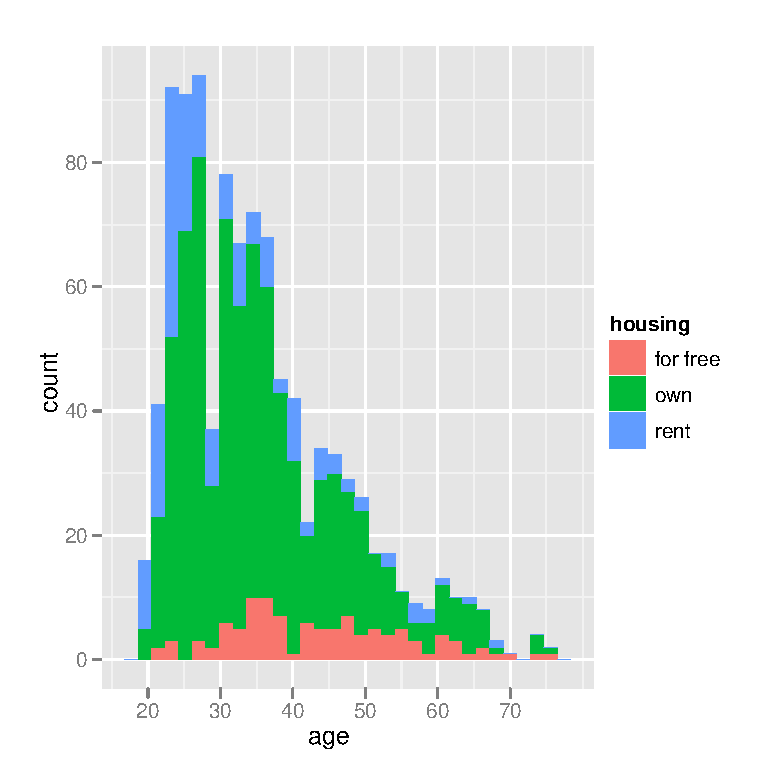
\includegraphics[keepaspectratio,width=7cm]{theimg/gg-foo14}}
 \hspace{0.1cm}
 \subfigure[gg-foo15]{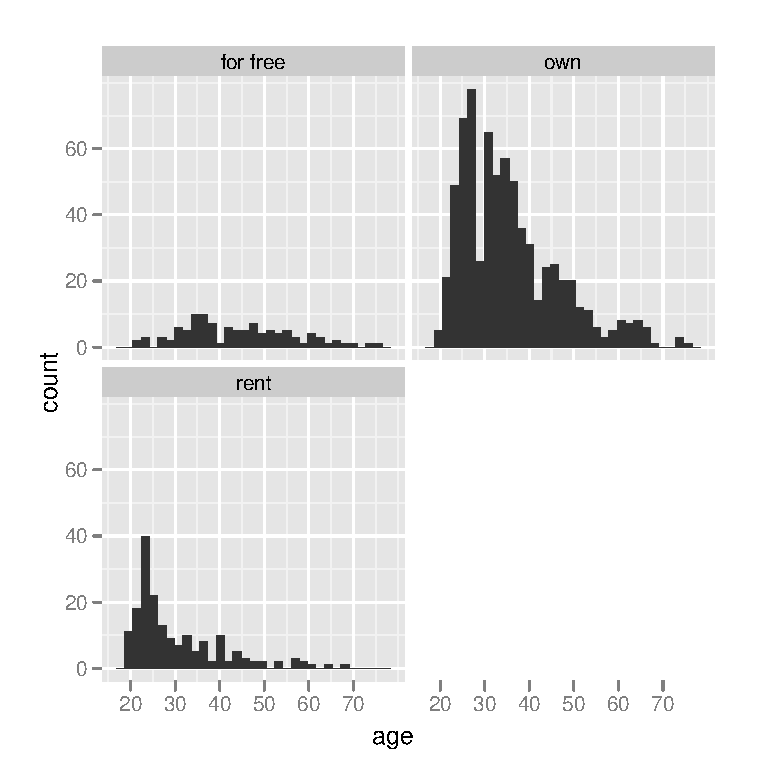
\includegraphics[keepaspectratio,width=7cm]{theimg/gg-foo15}}
 \caption{Barras y facetas}
 \label{fig:barras}
 \end{center}
\end{figure}



